\documentclass[11pt]{article}
\usepackage[a4paper,margin=2.5cm]{geometry}
\usepackage[T1]{fontenc}
\usepackage{lmodern}
\usepackage{microtype}
\usepackage{amsmath}
\usepackage{booktabs}
\usepackage{graphicx}
\usepackage{xcolor}
\usepackage{tabularx}
\usepackage{enumitem}
\usepackage[round,authoryear]{natbib}
\usepackage[hidelinks]{hyperref}
\usepackage{xurl}
\usepackage{caption}
\usepackage{subcaption}
\usepackage[section]{placeins}
\captionsetup{font=small,labelfont=bf}
\setlist{nosep,leftmargin=*}

% Auto-generated by paper/analysis.py — do not edit.
\newcommand{\dExtra}{74}
\newcommand{\dExtraPairs}{27}
\newcommand{\dOverDex}{1.73}
\newcommand{\thetaCritSixtyFour}{8.9M}
\newcommand{\thetaCritOneTwentyEight}{29.6M}
\newcommand{\thetaCritTwoFiftySix}{98.2M}
\newcommand{\thetaCritFiveTwelve}{326M}
\newcommand{\thetaCritOneM}{1.08B}
\newcommand{\thetaCritTwoM}{3.58B}
\newcommand{\tExtraTwoM}{27K}
\newcommand{\tExtraFiveM}{46K}
\newcommand{\tExtraEightM}{60K}
\newcommand{\tExtraSixteenM}{90K}
\newcommand{\tExtraThirtyTwoM}{134K}
\newcommand{\tExtraSixtyFourM}{200K}
\newcommand{\lamMaxEightM}{39.2M}
\newcommand{\lamRatioEightM}{299}
\newcommand{\accVOne}{61}
\newcommand{\accFracVOne}{99/161}
\newcommand{\dzVOne}{0}
\newcommand{\dzFracVOne}{0/40}
\newcommand{\dhVOne}{93}
\newcommand{\dhFracVOne}{28/30}
\newcommand{\nLangsVOne}{4}
\newcommand{\accDataA}{79}
\newcommand{\accFracDataA}{79/100}
\newcommand{\dzDataA}{0}
\newcommand{\dzFracDataA}{0/20}
\newcommand{\dhDataA}{100}
\newcommand{\dhFracDataA}{20/20}
\newcommand{\nLangsDataA}{2}
\newcommand{\accDataB}{81}
\newcommand{\accFracDataB}{81/100}
\newcommand{\dzDataB}{5}
\newcommand{\dzFracDataB}{1/20}
\newcommand{\dhDataB}{100}
\newcommand{\dhFracDataB}{20/20}
\newcommand{\nLangsDataB}{2}
\newcommand{\accThEight}{79}
\newcommand{\accFracThEight}{88/112}
\newcommand{\dzThEight}{20}
\newcommand{\dzFracThEight}{6/30}
\newcommand{\dhThEight}{100}
\newcommand{\dhFracThEight}{20/20}
\newcommand{\nLangsThEight}{3}
\newcommand{\accThSixteen}{95}
\newcommand{\accFracThSixteen}{104/110}
\newcommand{\dzThSixteen}{80}
\newcommand{\dzFracThSixteen}{24/30}
\newcommand{\dhThSixteen}{100}
\newcommand{\dhFracThSixteen}{20/20}
\newcommand{\nLangsThSixteen}{3}
\newcommand{\accThThirtyTwo}{100}
\newcommand{\accFracThThirtyTwo}{492/494}
\newcommand{\dzThThirtyTwo}{100}
\newcommand{\dzFracThThirtyTwo}{102/102}
\newcommand{\dhThThirtyTwo}{98}
\newcommand{\dhFracThThirtyTwo}{96/98}
\newcommand{\nLangsThThirtyTwo}{15}
\newcommand{\accVThree}{100}
\newcommand{\accFracVThree}{450/450}
\newcommand{\dzVThree}{100}
\newcommand{\dzFracVThree}{90/90}
\newcommand{\dhVThree}{100}
\newcommand{\dhFracVThree}{90/90}
\newcommand{\nLangsVThree}{15}
\newcommand{\accPrelude}{96}
\newcommand{\accFracPrelude}{432/450}
\newcommand{\dzPrelude}{98}
\newcommand{\dzFracPrelude}{88/90}
\newcommand{\dhPrelude}{89}
\newcommand{\dhFracPrelude}{80/90}
\newcommand{\nLangsPrelude}{15}
\newcommand{\accPreludeTwo}{96}
\newcommand{\accFracPreludeTwo}{288/300}
\newcommand{\dzPreludeTwo}{97}
\newcommand{\dzFracPreludeTwo}{58/60}
\newcommand{\dhPreludeTwo}{90}
\newcommand{\dhFracPreludeTwo}{54/60}
\newcommand{\nLangsPreludeTwo}{10}
\newcommand{\accTwoFiftySix}{89}
\newcommand{\accFracTwoFiftySix}{154/174}
\newcommand{\dzTwoFiftySix}{94}
\newcommand{\dzFracTwoFiftySix}{49/52}
\newcommand{\dhTwoFiftySix}{87}
\newcommand{\dhFracTwoFiftySix}{27/31}
\newcommand{\nLangsTwoFiftySix}{10}
\newcommand{\swDzThEight}{20}
\newcommand{\swDzFracThEight}{6/30}
\newcommand{\swDzLoThEight}{10}
\newcommand{\swDzHiThEight}{37}
\newcommand{\swSixtyFourDzThEight}{30/30}
\newcommand{\swDzThSixteen}{80}
\newcommand{\swDzFracThSixteen}{24/30}
\newcommand{\swDzLoThSixteen}{63}
\newcommand{\swDzHiThSixteen}{90}
\newcommand{\swSixtyFourDzThSixteen}{30/30}
\newcommand{\swDzThThirtyTwo}{100}
\newcommand{\swDzFracThThirtyTwo}{30/30}
\newcommand{\swDzLoThThirtyTwo}{89}
\newcommand{\swDzHiThThirtyTwo}{100}
\newcommand{\swSixtyFourDzThThirtyTwo}{30/30}
\newcommand{\pEightSixteen}{<0.001}
\newcommand{\pSixteenThirtyTwo}{=0.024}
\newcommand{\nSweepTrials}{30}
\newcommand{\sweepTokens}{294M}
\newcommand{\belowChancePVOne}{1e-05}
\newcommand{\belowChancePDataA}{0.003}
\newcommand{\belowChancePDataB}{0.02}
\newcommand{\dataA}{0/20}
\newcommand{\dataB}{1/20}
\newcommand{\dataAquarter}{19/20}
\newcommand{\dataBquarter}{20/20}
\newcommand{\vOneSixtyFour}{3/10}
\newcommand{\vOneQuarter}{12/31}
\newcommand{\vOneHalf}{28/30}
\newcommand{\ctrlNoCtx}{29\% (137/478)}
\newcommand{\ctrlShuffled}{100\% (478/478)}
\newcommand{\ctrlShort}{100\% (478/478)}
\newcommand{\marginThEight}{\textminus 3.1}
\newcommand{\marginThSixteen}{+2.0}
\newcommand{\marginThThirtyTwo}{+4.6}
\newcommand{\marginVOne}{\textminus 8.0}
\newcommand{\nRatioTrials}{2{,}445}
\newcommand{\ratioBelowOne}{97\% (1954/2005)}
\newcommand{\ratioOneToOneHalf}{92\% (219/237)}
\newcommand{\ratioOneHalfToTwo}{87\% (72/83)}
\newcommand{\ratioAboveTwo}{7\% (8/120)}
\newcommand{\ratioFiveTwelve}{2.5}
\newcommand{\ratioOneM}{4.2}
\newcommand{\lenExponent}{1.73}
\newcommand{\octaveFactor}{3.32}
\newcommand{\pMiddle}{=0.001}
\newcommand{\midVthree}{100\% (270/270)}
\newcommand{\midPrelude}{94\% (254/270)}
\newcommand{\midPreludePct}{94}
\newcommand{\midVthreePct}{100}
\newcommand{\pMid}{<0.001}
\newcommand{\halfPreludeSame}{51/60}
\newcommand{\halfPreludeTwo}{54/60}
\newcommand{\prelTwoIters}{300}
\newcommand{\prelTwoPlanned}{476}
\newcommand{\prelMidLangsImperfect}{6}
\newcommand{\prelMidLangs}{15}
\newcommand{\tfsZero}{94\% (49/52)}
\newcommand{\tfsQuarter}{79\% (37/47)}
\newcommand{\tfsHalf}{87\% (27/31)}
\newcommand{\tfsAll}{89\% (154/174)}
\newcommand{\tfsLangs}{10}
\newcommand{\tfsAtOneTwentyEight}{99\% (79/80)}
\newcommand{\tfsRatioZero}{1.28}


\hypersetup{
  pdftitle={The Start of the Window: RoPE's Critical Dimension Predicts the Base Frequency Needed for 128K--256K Context Extension},
  pdfauthor={Birger Mo\"ell},
  pdfsubject={Long-context extension of language models},
  pdfkeywords={long context, RoPE, rotary position embedding, base frequency, ABF, needle in a haystack, context extension, OpenEuroLLM}
}

\title{\textbf{The Start of the Window: RoPE's Critical Dimension Predicts the Base Frequency Needed for 128K--256K Context Extension}}
\author{Birger Mo\"ell\\[2pt]
\small AI Sweden\\
\small \url{https://github.com/BirgerMoell/openeuro-longctx-datamix}}
\date{November 2026 \quad (Version 1.0)}

\begin{document}
\maketitle

\begin{abstract}
\noindent
When a language model pretrained at 4K tokens is extended to 128K by raising the RoPE base frequency $\theta$ and continuing pretraining, it can retrieve facts from the middle and end of the window yet fail almost completely on facts placed at its very start. We study this \emph{depth-0} failure in a 9B-parameter multilingual OpenEuroLLM model extended to 128K and 256K tokens, using a forced-choice needle-in-a-haystack test in up to 15 languages and 20--90 trials per cell. Three results stand out. First, data does not fix it: two length-biased data mixes leave depth-0 accuracy at 64K at \dataA{} and \dataB{}, \emph{below} the 25\% chance level, because the model is drawn to distractors seen recently. Second, $\theta$ does: in a controlled sweep from one 64K checkpoint, with identical data and \sweepTokens{} tokens per arm, depth-0 accuracy at 128K rises from \swDzThEight\% ($\theta{=}8$M) to \swDzThSixteen\% (16M) to \swDzThThirtyTwo\% (32M). Third, the critical-dimension theory of RoPE extrapolation \citep{liu2024scalinglaws} predicts these thresholds without fitting: with a 4K pretraining window and base $10^5$, only the first \dExtra{} of 128 rotary dimensions complete a rotation in pretraining, giving a critical base of \thetaCritSixtyFour{} at 64K, \thetaCritOneTwentyEight{} at 128K and \thetaCritTwoFiftySix{} at 256K. Pooled over all runs, retrieval is \ratioBelowOne{} accurate when the needle lies within the critical period and \ratioAboveTwo{} beyond twice it. The theory implies that the critical base grows by a factor of \octaveFactor{} per doubling of context, not 2, so the common ``double $\theta$ per octave'' heuristic under-provisions 512K and 1M models by \ratioFiveTwelve$\times$ and \ratioOneM$\times$. A more-pretrained 1T-token base, extended with an identical recipe, fixes depth-0 but loses accuracy in the middle of the window (\midPreludePct\% versus \midVthreePct\% of mid-window trials correct), which a 1.26$\times$ token budget did not repair. We release the models, raw trials, launch scripts and analysis code.
\end{abstract}

\section{Introduction}

Rotary position embeddings \citep[RoPE;][]{su2024roformer} encode position by rotating pairs of query and key dimensions at frequencies $\theta^{-2i/d}$. A model pretrained at a short context can be extended by changing those frequencies and continuing pretraining on longer sequences: position interpolation \citep{chen2023pi}, NTK-aware scaling \citep{bloc97ntk}, YaRN \citep{peng2024yarn}, LongRoPE \citep{ding2024longrope,shang2025longrope2} and, the simplest, \emph{adjusted base frequency} (ABF), which raises the base $\theta$ \citep{xiong2024effective,roziere2023codellama,dubey2024llama3}. ABF needs one hyperparameter, yet practice varies widely: Code Llama uses $10^6$ for 100K tokens \citep{roziere2023codellama}, Llama~3 uses $5\times10^5$ \citep{dubey2024llama3}, and long-context recipes are often reported with little evidence on how $\theta$ was chosen \citep{fu2024data,gao2025prolong}.

We ran into the consequences of that choice while extending a multilingual 9B model for OpenEuroLLM \citep{openeurollm2025} from 4K to 128K tokens. With the base we first used ($5\times10^6$), the model retrieved needles from the second half of a 128K window perfectly and from the first quarter not at all. More long-document data did not help. Raising $\theta$ did. This report documents that diagnosis and asks whether the $\theta$ needed can be predicted. Our contributions are:
\begin{itemize}
\item \textbf{A controlled $\theta$ sweep} at 128K from a single 64K checkpoint, varying only $\theta$, with matched evaluation in three languages and confirmation in 15 (\S\ref{sec:sweep}).
\item \textbf{Evidence that the far-position failure is not a data problem}: two length-biased mixtures leave it intact, and failing models score \emph{below chance} because of how they fail (\S\ref{sec:data}).
\item \textbf{A parameter-free prediction}: the critical-dimension theory of \citet{liu2024scalinglaws}, evaluated with this model's pretraining base, length and head dimension, places the critical $\theta$ between the failing and succeeding runs at 64K, 128K and 256K, and orders all \nRatioTrials{} long-context trials by a single ratio (\S\ref{sec:theory}). It implies a steeper scaling than the ``double $\theta$ per octave'' rule we had been using (\S\ref{sec:predictions}).
\item \textbf{A base-model effect}: with an identical recipe, a 1T-token base fixes depth-0 but retains a lost-in-the-middle dip that a 0.6T-token base does not (\S\ref{sec:base}).
\item \textbf{Open artifacts}: four 128K/256K base models, every trial with its log-likelihoods, the launch scripts and the script that produces every number here (\S\ref{sec:availability}).
\end{itemize}

\section{Background and related work}
\label{sec:related}

\paragraph{RoPE and its wavelengths.} For head dimension $d$, RoPE rotates dimension pair $i\in\{0,\dots,d/2-1\}$ by angle $m\,\theta^{-2i/d}$ at position $m$, so pair $i$ has wavelength $\lambda_i=2\pi\theta^{2i/d}$. Low pairs rotate fast and encode local order; high pairs rotate slowly and encode long-range position.

\paragraph{Critical dimension.} \citet{liu2024scalinglaws} observe that during pretraining at length $T_{\mathrm{train}}$ with base $\theta_0$, only pairs whose wavelength is shorter than $T_{\mathrm{train}}$ see a complete rotation; the remaining, higher pairs only see a fraction of their period and learn position-dependent features that do not generalize. The boundary is the \emph{critical dimension} (their Lemma~1, stated for $\theta_0=10^4$; we use the model's own pretraining base)
\begin{equation}
d_{\mathrm{extra}} = 2\left\lceil \frac{d}{2}\log_{\theta_0}\frac{T_{\mathrm{train}}}{2\pi}\right\rceil .
\label{eq:dextra}
\end{equation}
For a larger base $\theta$ applied while tuning at the original length, the model can only extrapolate as far as the new period of the critical dimension (their Theorem~2),
\begin{equation}
T_{\mathrm{extra}}(\theta) = 2\pi\,\theta^{\,d_{\mathrm{extra}}/d}.
\label{eq:textra}
\end{equation}
Their Theorem~3 extends the analysis to tuning at a longer length $T_{\mathrm{tune}}$: if $\theta$ is below a critical value, tuning at $T_{\mathrm{tune}}$ is predicted to train the formerly incomplete dimensions and the reach becomes $T_{\mathrm{tune}}$ itself. \citet{men2024base} derive a different lower bound on the base from the requirement that attention can still distinguish similar from random keys at every distance, solved numerically per context length. Other analyses attribute ABF's far-distance behaviour to attention patterns \citep{zhong2024attention}, round wavelengths to avoid out-of-distribution gaps \citep{wang2024resonance}, and motivate searching per-dimension scales \citep{shang2025longrope2}. Positional schemes without RoPE \citep{press2022alibi,kazemnejad2023nope} avoid the problem but are not what most current models use.

\paragraph{Long-context training and evaluation.} Data engineering for 128K contexts \citep{fu2024data} and systematic recipes \citep{gao2025prolong} emphasize long-document data and short-context retention. Effective context is often shorter than the trained window \citep{an2025string}, and models use the middle of the context worse than its ends \citep{liu2024lostmiddle}. Needle-in-a-haystack tests \citep{kamradt2023niah} are the simplest diagnostic; RULER and HELMET give broader coverage \citep{hsieh2024ruler,yen2025helmet}. We use a forced-choice variant that works on base models and isolates retrieval by depth.

\section{Setup}
\label{sec:setup}

\paragraph{Model.} The OpenEuroLLM 9B dense base model \citep{openeurollm2025} has 36 layers, hidden size 4096, 32 query and 8 key--value heads with head dimension $d=128$, full (non-partial) RoPE, a multilingual 263K-entry tokenizer, and was pretrained at $T_{\mathrm{train}}=4096$ with $\theta_0=10^5$. We extend two checkpoints of the same pretraining run: one after about 0.6T tokens and \emph{Prelude}, after about 1T tokens.

\paragraph{Extension recipe.} Native ABF in stages: each stage loads the previous checkpoint, raises the sequence length and $\theta$, and continues pretraining with Megatron-LM \citep{shoeybi2019megatron} and FlashAttention \citep{dao2024flashattention2} on LUMI (AMD MI250X), with tensor parallelism 8 and context parallelism 2--16 \citep{liu2024ringattention}; global batch 64 sequences, AdamW, learning rate $10^{-5}$ with cosine decay to $10^{-6}$ (the 256K stage: $8\times10^{-6}$). The chain is 16K ($\theta{=}5\times10^5$) $\to$ 32K ($10^6$) $\to$ 64K ($2\times10^6$, 2--3B tokens) $\to$ 128K $\to$ 256K. Data is a multilingual long-context mix of about 150 sources (``length-biased A''), an alternative mix with 65\% length-filtered long documents (``length-biased B''), or the original catalogue mix (v1); the 256K stage adds 60\% concatenated genuinely long documents. Table~\ref{tab:runs} lists every evaluated checkpoint.

\paragraph{Evaluation.} We use a base-model, forced-choice needle-in-a-haystack test (\nolinkurl{scripts/eval_base_lm_niah.py}). A context of the target length is filled with lines of the form ``The special magic number for \emph{key} is: \emph{value}.'' in the test language, cycling about 50 key--value pairs. The query line, for a key that appears exactly once, is inserted at relative depth $d\in\{0, 0.25, 0.5, 0.75, 1\}$ ($d{=}0$: directly after a one-line preamble). The context ends with the query prefix, and the model scores four candidate values by total log-likelihood: the true value and three values bound to \emph{other} keys in the same context, which therefore appear many times throughout it. Chance is 25\%. Three controls check the harness: with no context (expected $\approx$25\%), with all bindings rotated so the correct answer changes, and with a 256-token context. Languages are drawn from the 15 for which templates were written (English, German, French, Spanish, Dutch, Polish, Swedish, Finnish, Czech, Italian, Portuguese, Greek, Hungarian, Ukrainian, Danish); early runs used French, Finnish, Czech and Dutch. Each $(\text{language}, \text{depth}, \text{trial})$ case is seeded deterministically, so the same cases recur across models and duplicated cases across jobs are counted once. Intervals are Wilson 95\% intervals \citep{wilson1927}; two-proportion comparisons use Fisher's exact test \citep{agresti2002}.

\begin{table}[htbp]
\centering
\small
\caption{Every evaluated checkpoint and its accuracy by needle depth at its evaluation length $L$ (all evaluated languages pooled). Tokens: tokens in the final stage. The three sweep arms start from the same 64K checkpoint (length-biased A).}
\label{tab:runs}
\resizebox{\linewidth}{!}{\begin{tabular}{lrrrrrrrrrr}
\toprule
Run & $\theta$ & Eval $L$ & Base & Tokens & Lang. & $d=0.0$ & $d=0.25$ & $d=0.5$ & $d=0.75$ & $d=1.0$ \\
\midrule
v1 (catalogue data) & 5M & 128K & 0.6T & 1.00B & 4 & 0 (0/40) & 39 (12/31) & 93 (28/30) & 97 (29/30) & 100 (30/30) \\
64K, length-biased A & 2M & 64K & 0.6T & 3.00B & 2 & 0 (0/20) & 95 (19/20) & 100 (20/20) & 100 (20/20) & 100 (20/20) \\
64K, length-biased B & 2M & 64K & 0.6T & 3.00B & 2 & 5 (1/20) & 100 (20/20) & 100 (20/20) & 100 (20/20) & 100 (20/20) \\
sweep θ=8M & 8M & 128K & 0.6T & 0.29B & 3 & 20 (6/30) & 100 (22/22) & 100 (20/20) & 100 (20/20) & 100 (20/20) \\
sweep θ=16M & 16M & 128K & 0.6T & 0.29B & 3 & 80 (24/30) & 100 (20/20) & 100 (20/20) & 100 (20/20) & 100 (20/20) \\
sweep θ=32M & 32M & 128K & 0.6T & 0.29B & 15 & 100 (102/102) & 100 (98/98) & 98 (96/98) & 100 (98/98) & 100 (98/98) \\
v3 θ=32M (0.6T base) & 32M & 128K & 0.6T & 2.00B & 15 & 100 (90/90) & 100 (90/90) & 100 (90/90) & 100 (90/90) & 100 (90/90) \\
Prelude θ=32M (1T base) & 32M & 128K & 1T & 2.00B & 15 & 98 (88/90) & 97 (87/90) & 89 (80/90) & 97 (87/90) & 100 (90/90) \\
Prelude θ=32M, 1.26× tokens & 32M & 128K & 1T & 2.52B & 10 & 97 (58/60) & 98 (59/60) & 90 (54/60) & 95 (57/60) & 100 (60/60) \\
Prelude θ=64M, 256K & 64M & 256K & 1T & 0.99B & 10 & 94 (49/52) & 79 (37/47) & 87 (27/31) & 86 (19/22) & 100 (22/22) \\
\bottomrule
\end{tabular}
}
\end{table}

The controls behave as intended across all runs: \ctrlNoCtx{} without context, \ctrlShuffled{} with rotated bindings and \ctrlShort{} at 256 tokens.

\section{Results}

\subsection{More long data does not fix depth-0}
\label{sec:data}
Our first 128K model (v1, $\theta=5\times10^6$, catalogue mix) retrieved needles at depth $\ge0.5$ almost perfectly (\vOneHalf{} at $d{=}0.5$) but at depth 0 it scored \dzFracVOne{} and at depth 0.25 \vOneQuarter{} (Figure~\ref{fig:depth}). The natural explanation was too little genuinely long data. We therefore rebuilt the 64K stage with two length-biased mixtures, keeping $\theta=2\times10^6$. Both reached 100\% at depth $\ge0.5$ and failed at depth 0 just as before (\dataA{} and \dataB{} at 64K). Data composition did not move the failure.

\paragraph{Failing below chance.} These failures are not random guessing: \dzFracVOne{} is far below the 25\% chance rate (binomial $p=\belowChancePVOne$). In this test the three distractor values are bound to other keys that recur throughout the context, including just before the query, while the true value appears once. A model that cannot attend to the start of the window still has the recent, repeated distractors available and chooses one of them; the median log-likelihood margin of the true value over the best distractor is \marginVOne{} nats (Figure~\ref{fig:margins}). Below-chance accuracy is therefore a signature of a position-specific blind spot, and a reminder that single-needle tests with in-context distractors are adversarial by construction.

\begin{figure}[htbp]
\centering
\begin{subfigure}[t]{0.49\linewidth}
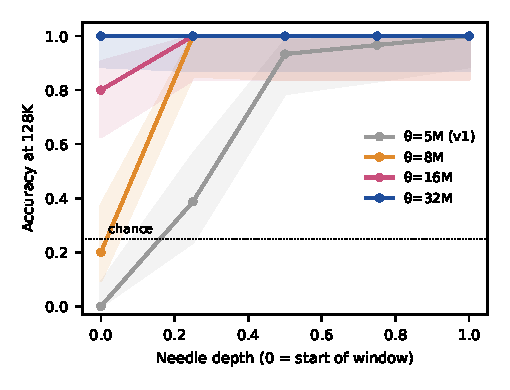
\includegraphics[width=\linewidth]{figures/depth_profiles.pdf}
\caption{Accuracy by depth at 128K (sweep: fr, fi, cs; $n=20$--30 per point). Shaded: Wilson 95\% CI.}
\label{fig:depth}
\end{subfigure}\hfill
\begin{subfigure}[t]{0.49\linewidth}
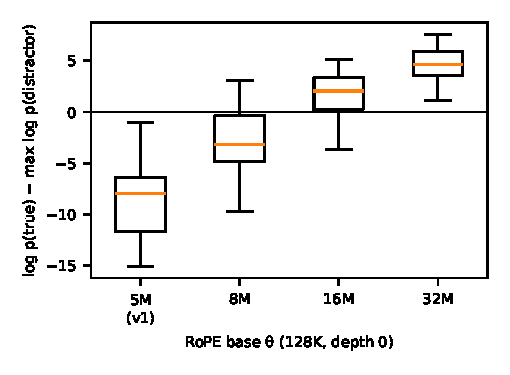
\includegraphics[width=\linewidth]{figures/margins.pdf}
\caption{Log-likelihood margin of the true value over the best distractor at depth 0, 128K.}
\label{fig:margins}
\end{subfigure}
\caption{Raising $\theta$ restores retrieval from the start of a 128K window.}
\end{figure}

\subsection{A controlled $\theta$ sweep}
\label{sec:sweep}
We then held everything but $\theta$ fixed. From the 64K checkpoint trained on length-biased mix A, three arms continued pretraining at 128K for 35 steps (\sweepTokens{} tokens) with $\theta$ = 8M, 16M and 32M and identical data, schedule and seed. Table~\ref{tab:sweep} and Figure~\ref{fig:depth} show the result. At 64K all three arms retrieve perfectly at every depth. At 128K, depth-0 accuracy rises from \swDzFracThEight{} (8M; 95\% CI \swDzLoThEight--\swDzHiThEight\%) to \swDzFracThSixteen{} (16M; \swDzLoThSixteen--\swDzHiThSixteen\%) to \swDzFracThThirtyTwo{} (32M; \swDzLoThThirtyTwo--\swDzHiThThirtyTwo\%). Both steps are significant (Fisher $p\pEightSixteen$ and $p\pSixteenThirtyTwo$), and the log-likelihood margin moves from \marginThEight{} to \marginThSixteen{} to \marginThThirtyTwo{} nats. Depths $\ge0.25$ are near-perfect for every arm, so the whole effect of $\theta$ is concentrated at the start of the window. Over all its evaluations, including all 15 languages, the 32M arm scored \dzFracThThirtyTwo{} at depth 0, and the same $\theta$ trained for 2B tokens (v3) scored \accFracVThree{} overall.

\begin{table}[htbp]
\centering
\small
\caption{Controlled $\theta$ sweep: accuracy (\%) by depth for three arms continued from one 64K checkpoint with identical data and \sweepTokens{} tokens (French, Finnish, Czech; 20--30 trials per cell). $T_{\mathrm{extra}}$: Eq.~\ref{eq:textra}.}
\label{tab:sweep}
\resizebox{\linewidth}{!}{\begin{tabular}{rrrrrrrrrrrrr}
\toprule
 & & \multicolumn{5}{c}{Evaluated at 64K} & \multicolumn{5}{c}{Evaluated at 128K} & \\
\cmidrule(lr){3-7}\cmidrule(lr){8-12}
$\theta$ & $T_{\mathrm{extra}}$ & 0.0 & 0.25 & 0.5 & 0.75 & 1.0 & 0.0 & 0.25 & 0.5 & 0.75 & 1.0 & 95\% CI $d=0$ \\
\midrule
8M & 60K & 100 & 100 & 100 & 100 & 100 & 20 & 100 & 100 & 100 & 100 & [10, 37] \\
16M & 90K & 100 & 100 & 100 & 100 & 100 & 80 & 100 & 100 & 100 & 100 & [63, 90] \\
32M & 134K & 100 & 100 & 100 & 100 & 100 & 100 & 100 & 100 & 100 & 100 & [89, 100] \\
\bottomrule
\end{tabular}
}
\end{table}

Note that $\theta=8$M already gives the slowest RoPE pair a wavelength of \lamMaxEightM{} tokens, \lamRatioEightM{} times the 128K window. A criterion based on the longest wavelength alone (``every position gets a distinct angle'') would therefore call 8M more than sufficient. It is not: what matters is not the slowest dimension but the slowest dimension the model has learned to use.

\subsection{The critical dimension predicts the threshold}
\label{sec:theory}
For this model, Eq.~\ref{eq:dextra} with $d=128$, $\theta_0=10^5$ and $T_{\mathrm{train}}=4096$ gives $d_{\mathrm{extra}}=\dExtra$: the top \dExtraPairs{} of the 64 rotary pairs never completed a rotation during pretraining. Eq.~\ref{eq:textra} then gives the reach of each base: \tExtraTwoM{} tokens for $\theta=2$M, \tExtraFiveM{} for 5M, \tExtraEightM{} for 8M, \tExtraSixteenM{} for 16M, \tExtraThirtyTwoM{} for 32M and \tExtraSixtyFourM{} for 64M. Inverting it, the smallest base whose critical period covers $L$ tokens is
\begin{equation}
\theta_{\mathrm{crit}}(L) = \left(\frac{L}{2\pi}\right)^{d/d_{\mathrm{extra}}},
\label{eq:thetacrit}
\end{equation}
which is \thetaCritSixtyFour{} at 64K, \thetaCritOneTwentyEight{} at 128K and \thetaCritTwoFiftySix{} at 256K. These values, computed from the pretraining configuration alone, separate our runs (Figure~\ref{fig:theta}): at 64K, the 2M checkpoints fail and the 8M arm (just below 8.9M), evaluated at 64K, succeeds; at 128K, 5M and 8M fail, 16M is partial and 32M (just above 29.6M) is perfect; at 256K, 64M (below 98M) reaches \tfsZero{} at depth 0, good but not perfect.

\begin{figure}[htbp]
\centering
\begin{subfigure}[t]{0.49\linewidth}
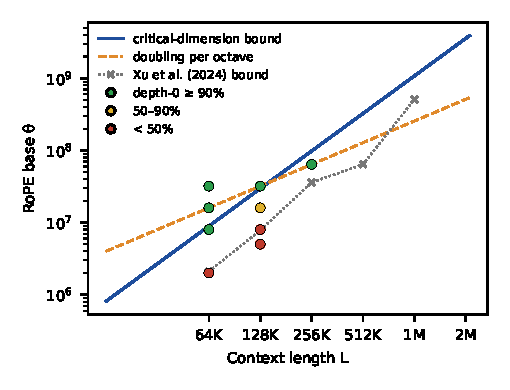
\includegraphics[width=\linewidth]{figures/theta_vs_length.pdf}
\caption{Every evaluated run at its length and base, coloured by depth-0 accuracy, against Eq.~\ref{eq:thetacrit} and the doubling rule.}
\label{fig:theta}
\end{subfigure}\hfill
\begin{subfigure}[t]{0.49\linewidth}
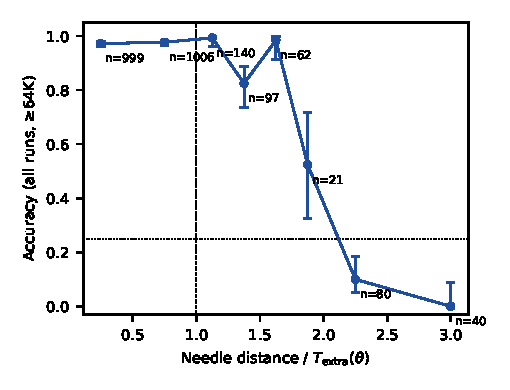
\includegraphics[width=\linewidth]{figures/distance_ratio.pdf}
\caption{Accuracy against needle distance divided by $T_{\mathrm{extra}}(\theta)$, pooling every main-condition trial at $\ge$64K across all runs.}
\label{fig:ratio}
\end{subfigure}
\caption{The critical-dimension period organizes all long-context results.}
\end{figure}

Two features of this result deserve emphasis. First, we apply the bound of Eq.~\ref{eq:textra}, derived for tuning at the original length, although our models were tuned \emph{at} the target length. Liu et al.'s Theorem~3 predicts that tuning at the target length should lift the reach to that length for any sufficiently small base, which would make $\theta=8$M adequate at 128K. Our runs say otherwise: 0.3--3B tokens of tuning at 64K or 128K did not teach the under-trained dimensions to represent the new distances, and the pretraining-length bound is what separates success from failure. Second, the numerical bound of \citet{men2024base}---7.8M for 128K and 36M for 256K---is met by our failing 8M run at 128K; it is a necessary condition in our data but not a sufficient one.

A stronger test uses every trial, not only depth 0. For each trial we divide the distance between the needle and the query, $(1-\text{depth})\times L$, by $T_{\mathrm{extra}}(\theta)$ of the model that answered it. Figure~\ref{fig:ratio} pools all runs, data mixes, budgets, bases and languages. Accuracy is \ratioBelowOne{} for ratios below 1, \ratioOneToOneHalf{} between 1 and 1.5, \ratioOneHalfToTwo{} between 1.5 and 2, and \ratioAboveTwo{} beyond 2. A single quantity from the pretraining configuration explains where retrieval breaks across 64K--256K, three data mixtures and two bases. The empirical edge lies somewhat beyond the bound (retrieval degrades between 1.5 and 2 rather than at 1), so Eq.~\ref{eq:thetacrit} is a safe rather than a tight choice; partly trained dimensions beyond $d_{\mathrm{extra}}$ evidently still carry some usable signal.

\subsection{Implications for longer contexts}
\label{sec:predictions}
Eq.~\ref{eq:thetacrit} implies $\theta_{\mathrm{crit}}\propto L^{d/d_{\mathrm{extra}}}=L^{\lenExponent}$: each doubling of the context multiplies the critical base by $2^{\lenExponent}\approx\octaveFactor$, not 2. Our working rule (``the critical $\theta$ doubles per octave'', anchored at 32M for 128K) was consistent with 64K and 128K but already undershoots at 256K, where the 64M model is the one run below the line, and the gap widens (Table~\ref{tab:pred}): for 512K the theory asks for \thetaCritFiveTwelve{} rather than 128M, and for 1M \thetaCritOneM{} rather than 256M. These are predictions, not measurements; they also assume that the 4K pretraining configuration still governs, which further long-context training at intermediate lengths may change.

\begin{table}[htbp]
\centering
\small
\caption{Critical base from Eq.~\ref{eq:thetacrit} for this model ($d=128$, $\theta_0=10^5$, $T_{\mathrm{train}}=4096$), the lower bound of \citet[Table~1]{men2024base}, and the doubling rule anchored at 32M for 128K.}
\label{tab:pred}
\begin{tabular}{lrrrr}
\toprule
$L$ & $\theta_{\mathrm{crit}}$ (Eq.~\ref{eq:thetacrit}) & Bound of \citet{men2024base} & Doubling rule & Ratio to doubling \\
\midrule
64K & 8.9M & 2.1M & 16M & 0.6$\times$ \\
128K & 29.6M & 7.8M & 32M & 0.9$\times$ \\
256K & 98.2M & 36M & 64M & 1.5$\times$ \\
512K & 326M & 64M & 128M & 2.5$\times$ \\
1M & 1.08B & 510M & 256M & 4.2$\times$ \\
2M & 3.58B & -- & 512M & 7.0$\times$ \\
\bottomrule
\end{tabular}

\end{table}

\subsection{A more-pretrained base resists flattening the middle}
\label{sec:base}
We repeated the 128K recipe exactly---same $\theta$ (32M), data, schedule and 2B-token budget---on Prelude, the same pretraining run at 1T rather than 0.6T tokens. Depth 0 is fixed (\dzFracPrelude), as the theory predicts for an identical $\theta$. But accuracy in the middle of the window falls: \dhFracPrelude{} at depth 0.5 versus \dhFracVThree{} for the 0.6T base, and \midPrelude{} versus \midVthree{} pooled over depths 0.25--0.75 (Fisher $p\pMid$; Figure~\ref{fig:base}). The dip appears in \prelMidLangsImperfect{} of \prelMidLangs{} languages. Continuing training to 300 of a planned 476 steps (1.26$\times$ the tokens; the job hit its wall-clock limit) did not remove it: \halfPreludeTwo{} at depth 0.5 versus \halfPreludeSame{} for the 2B-token model on the same \nLangsPreludeTwo{} languages.

\begin{figure}[htbp]
\centering
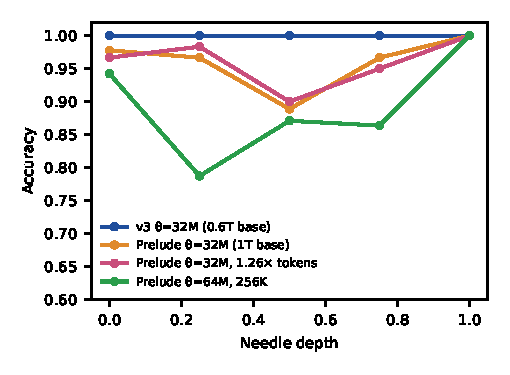
\includegraphics[width=0.55\linewidth]{figures/base_comparison.pdf}
\caption{Accuracy by depth for the 0.6T-token base (v3), the 1T-token Prelude base with the same recipe, Prelude with 1.26$\times$ tokens, and the 256K Prelude model (evaluated at 256K).}
\label{fig:base}
\end{figure}

Because data, $\theta$, budget, schedule, evaluation cases and conversion pipeline are identical between the two 128K runs, the base checkpoint is the remaining difference. A plausible reading is that a longer-pretrained model has a more entrenched preference for the beginning and end of its context \citep{liu2024lostmiddle} that a short extension phase does not undo; the 1.26$\times$ run argues that modestly more tokens are not enough, but it does not rule out a larger budget, a higher learning rate, or data that places relevant content mid-context. We report this as an open observation.

\paragraph{256K.} Extending the 128K Prelude model to 256K with $\theta=64$M and 1B tokens gives \tfsAll{} at 256K over \tfsLangs{} languages, with \tfsZero{} at depth 0, \tfsQuarter{} at depth 0.25 and \tfsHalf{} at depth 0.5, while keeping \tfsAtOneTwentyEight{} at 128K. Its depth-0 distance is \tfsRatioZero{} times $T_{\mathrm{extra}}(64\text{M})$, inside the region where Figure~\ref{fig:ratio} predicts high but imperfect accuracy; the theory's recommendation for 256K is about 98M. The 256K evaluation is small (\accFracTwoFiftySix{} trials) and should be read as preliminary.

\section{Discussion}
\label{sec:discussion}

\paragraph{Diagnosing a long-context failure.} A depth-stratified evaluation separates two failure types that an aggregate needle score conflates. A failure concentrated at the start of the window, sharp in depth and resistant to more data, points to the position encoding; a soft dip in the middle points elsewhere (training budget, base model, data placement). In our runs the first responded only to $\theta$; the second appeared with $\theta$ held fixed and depended on the base checkpoint.

\paragraph{Choosing $\theta$.} For a RoPE model pretrained at $T_{\mathrm{train}}$ with base $\theta_0$ and head dimension $d$, Eqs.~\ref{eq:dextra}--\ref{eq:thetacrit} give a principled starting point before any extension run. For models like ours (4K, $10^5$, $d{=}128$) that means roughly 9M at 64K, 30M at 128K and 100M at 256K. Models pretrained with a longer window or a larger base have a larger $d_{\mathrm{extra}}$ and a gentler exponent; models with partial rotary embeddings or other head dimensions need the formula recomputed, which may explain why bases that work for one family look too small or too large for another.

\paragraph{Why not more data?} Data matters for overall quality, the middle of the window and short-context retention \citep{fu2024data,gao2025prolong}, none of which this report measures. But under a fixed position encoding, additional long documents cannot make an untrained rotary dimension represent distances it never rotated through during pretraining; in our runs, data changes did not move depth-0 accuracy at all, while $\theta$ changes moved it from 20\% to 100\% with only \sweepTokens{} tokens.

\section{Limitations}
\begin{itemize}
\item \textbf{One diagnostic.} The needle test is synthetic, repetitive and single-needle. We did not run RULER, HELMET or long-document QA \citep{hsieh2024ruler,yen2025helmet}, and we did not measure short-context regression, which large bases can cause.
\item \textbf{Small samples and shared cases.} Cells have 20--90 trials. The evaluation script seeded trials by trial index, so trials in different languages share the same keys and values and differ only in the surrounding language; language-pooled intervals are therefore optimistic.
\item \textbf{One model family.} All results are for one 9B architecture with full RoPE and one pretraining configuration. The agreement with Eq.~\ref{eq:thetacrit} at three lengths is encouraging but is not a test across architectures.
\item \textbf{Confounds outside the sweep.} The $\theta$ sweep is controlled; other comparisons (v1, the 64K data variants, the two bases) differ in more than one factor, as stated. The 1T-base comparison changes only the base checkpoint, but the 1.26$\times$ run was cut short.
\item \textbf{Short sweep arms.} Sweep arms saw \sweepTokens{} tokens. That suffices to fix depth-0 at 32M, but longer training might lower the threshold somewhat; the 2B-token v3 run used the same $\theta$.
\item \textbf{Predictions beyond 256K are untested.} Table~\ref{tab:pred} is a hypothesis to be validated, not a recipe.
\end{itemize}

\section{Conclusion}
When a context-extended RoPE model cannot read the start of its window, the base frequency is the first thing to check. In a 9B multilingual model, length-biased data left the failure intact; raising $\theta$ fixed it in a controlled sweep; and the critical-dimension theory, computed from the pretraining configuration alone, predicted where the threshold lies at 64K, 128K and 256K and organized every long-context trial by a single distance ratio. It also implies that the critical base grows faster than the doubling rule commonly used, which matters for extensions to 512K and beyond.

\section*{Availability}
\label{sec:availability}
Models (Apache-2.0): \nolinkurl{birgermoell/oellm-9b-128k-theta32m} (32M sweep arm), \nolinkurl{birgermoell/oellm-9b-128k-theta32m-v3}, \nolinkurl{birgermoell/oellm-9b-128k-theta32m-prelude} and \nolinkurl{birgermoell/oellm-9b-256k-theta64m-prelude} on Hugging Face, mirrored under \nolinkurl{openeurollm/}. Raw per-trial results with log-likelihoods, launch scripts, the evaluation script and \nolinkurl{paper/analysis.py}, which produces every number, table and figure here, are at \url{https://github.com/BirgerMoell/openeuro-longctx-datamix}.

\section*{Acknowledgements}
Training and evaluation ran on the EuroHPC system LUMI. We thank the OpenEuroLLM consortium for the base models, Jouni Luoma for the long-context data mix and training scripts on which this work builds, and the OpenEuroLLM long-context group for discussion.

\bibliographystyle{plainnat}
\bibliography{references}

\end{document}
